\npchapter{Context at SAP Gardener}
As mentioned in the introduction, this work is written in cooperation with SAP. In fact, the limitations mentioned in the previous chapter are deducted from the limitations the SAP Gardener team struggles with themselves. Subsequently, this chapter introduces the \textit{Open Component Model (OCM)}, SAP Gardeners proposed standard to decouple the compliance scans from the CI/CD pipeline. Based on this knowledge, an overview of the development and deployment landscape of SAP Gardener is given. Finally, the suggested integration of the Security and Compliance Data Lake, as a central application for storing and querying software metadata, with the existing standard and landscape is presented. Thereby, this chapter provides a reference architecture on how to overcome the major limitations of the current state of the art approach. 

\section{Open Component Model}
The OCM is an SBOM format created and used by SAP Gardener. It does not fulfill the minimum requirements as defined by the NTIA. But this is due to the fact that the OCM has a different focus than SPDX or CycloneDX. While those two were deliberately designed to be a bill of materials, thoroughly listing the inventory of a software, the OCM was specifically developed to decouple CI from CD and thereby overcome related limitations such as the ones mentioned in the previous chapter. Following is a technical explanation of the OCM deducted from the specification \cite{OCMSpec} and an internal presentation \cite{OCMInternalPresentation}. Even though this explanation focuses on understanding the rationale behind the design decisions of the proposed standard rather than technical completeness, it may still be a little hard to grasp at times. This is due to the abstract nature of the OCM. Therefore, emphasis and examples are used where possible. Also, while the textual description really explains the OCM as the abstract model that it is, figure \ref{fig:ComponentDescriptor} below shows an actual \emph{Component Descriptor}, the serialization format of the OCM. This may also support in understanding the abstract concepts.\\\\

\begin{figure}[H]
	\centering
	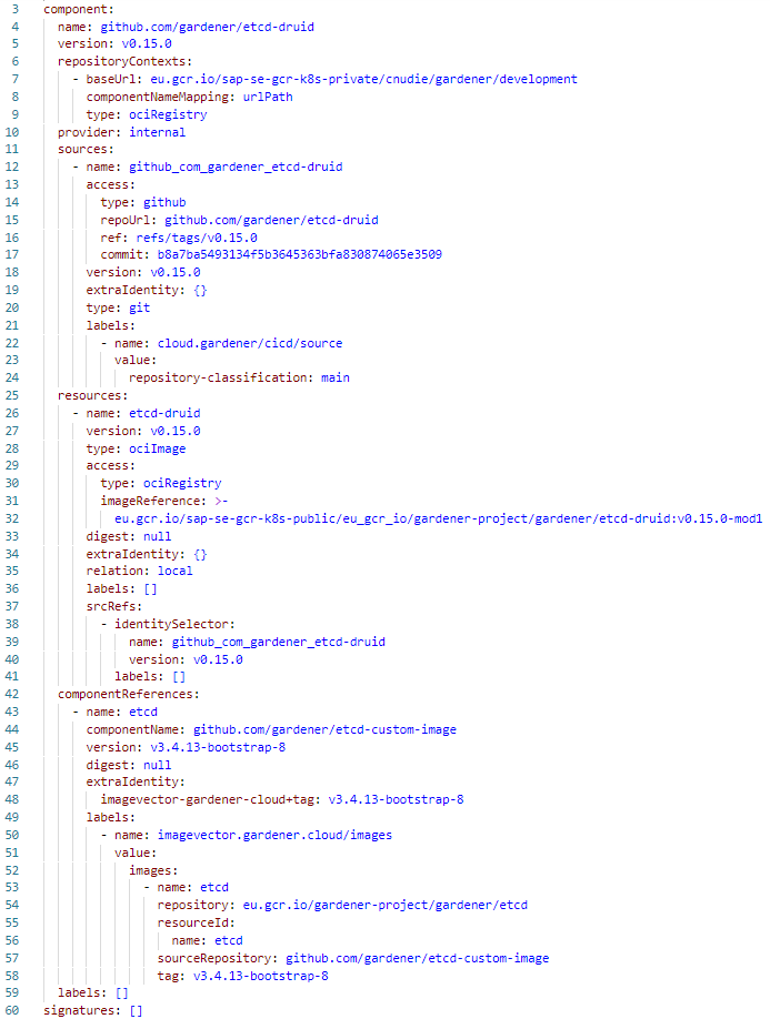
\includegraphics[scale=0.7]{componentdescriptor}
	\caption[Component Descriptor]{Component Descriptor \source{Based on \cite{OCMSpec}}}
	\label{fig:ComponentDescriptor}
\end{figure}


\noindent In the context of the OCM, a \emph{Component} is a software intended for a purpose which is identified by a \emph{globally unique name}. This definition is still pretty vague. But this is on purpose and it will become clear why throughout this section.\par 
\noindent A \emph{Component Version} is identified by the \emph{globally unique name} of the corresponding \emph{Component} and a \emph{version}. A \emph{Component Version} may contain \emph{Component References} and \emph{Artifact References}. Furthermore, it has a \emph{Repository Context}, a \emph{Labels} and a \emph{Provider} property. \emph{Repository Context} provides a formal description of the repositories that store a representation of this \emph{Component Version} and how to access them. \emph{Labels} is really just a container for additional metadata. It therefore is an array of objects with the properties \emph{name} and \emph{value}. The \emph{name} is a string while \emph{value} may be a string, array or map, arbitrarily nested. \emph{Provider} specifies the company or organization providing the \emph{Component Version}.\par 
\noindent A \emph{Component Reference} is a reference to another \emph{Component Version}. This initially sounds simple but there is actually a pitfall. A \emph{Component Reference} is not identified by the \emph{Identity} of another \emph{Component Version}, thus by the \emph{globally unique name} and the \emph{version}. Each \emph{Component Reference} has a \emph{Component Version-local Identity} which additionally to the \emph{globally unique Identity} of the referenced \emph{Component Version} contains a \emph{name} and an \emph{extra identity}. This is due to the fact that a \emph{Component Reference} does not have a strict predefined semantic. An example might help to understand this. Imagine one \emph{Component Version} describing a version of a web server and another \emph{Component Version} describing a version of an entire landscape of a REST application (as already mentioned, the definition of a \emph{Component} is very loose). Now the REST application \emph{Component Version} may use the web server \emph{Component Version} twice, once as a classic HTTP server and once as a HTTP load balancer. Therefore, one \emph{Component Reference} could have the \emph{name} "http server" and the other "load balancer". Due to this definition of \emph{Component Reference Identity}, the OCM provides the semantic capabilities to express such a situation. If the \emph{name} is also not sufficient to uniquely identify a \emph{Component Reference} within a \emph{Component Version}, perhaps because the same \emph{Component Version} is used as a HTTP server twice, the \emph{extra identity} may be used to provide further distinction. This is a flat map of key-value-pairs. Besides, every \emph{Component References} may also have a container for additional metadata, thus a \emph{Labels} property.\par 
\noindent \emph{Artifact} is used as an umbrella term for \emph{Sources} and \emph{Resources}. \emph{Sources} are usually the input for the build process of \emph{Resources}, typically some source code. Subsequently, \emph{Resources} are usually built from \emph{Sources} and are capable of doing something. Thus, \emph{Resources} are typically executables or OCI Images. \emph{Artifact References} have a \emph{Component Version-local Identity}, similar to \emph{Component References}. There is one significant different between the two which may easily lead to confusion. In the \emph{Component Reference Identity}, the \emph{version} is part of the referenced \emph{Component Versions Identity}. In the \emph{Artifact Reference}, the \emph{version} is only part of the \emph{Artifact Reference Identity}. What this means in practice is, if the \emph{version} within a \emph{Component Reference} changes, it is actually referencing a different \emph{Component Version}. On the other hand, if the \emph{version} within a \emph{Artifact Reference} changes, the referenced \emph{Artifact}, so the executeable or OCI Images, may still be exactly the same. Reciprocal, even if the \emph{version} is the same in two \emph{Artifact References}, the referenced \emph{Artifacts} may have different versions. So there is no concrete coupling between the physical \emph{Artifact}, so the executeable or the OCI Image, and the \emph{Artifact Reference}. The \emph{version} here is just another property to semantically distinct \emph{Artifact References} within a \emph{Component Version}, like \emph{name} and \emph{extra identity}. As a consequence, a \emph{Artifact Reference} with the \emph{name} "web server and \emph{version} "v1.2.8" could reference an nginx v1.1.3 executeable and another \emph{Artifact Reference} within the same \emph{Component Version} with the \emph{name} "web server" and \emph{version} "v2.0.0" could reference an apache v2.4.54 executeable. This is an extreme case, supposed to show that there actually is now real coupling. In practice, the \emph{name} and \emph{version} usually do correspond to the underlying \emph{Artifact}. And to do further distinctions in cases where a \emph{Component Version} references the same physical \emph{Artifact} twice, as an example twice nginx v1.1.3, once as an executeable for ARM platforms and once for x86-based platforms, the \emph{extra identity} is used. The actual reference or rather coupling to the executeable or OCI Image is provided and \emph{access} properties of the \emph{Artifact Reference} .The \emph{access} property, which is a map of key-value-pairs which has a required \emph{type} property, provides a formal description of how and where to access the \emph{Artifact}. Thereby, the \emph{type} defines the access method, usually by specifying the repository type. The other key-values pairs in the map then depend on that type and may reference a particular commit by specifying the repository URL and a commit hash. Furthermore, all \emph{Artifact References} have a \emph{type} and \emph{Labels} property, and specifically \emph{Resource References} additionally have a \emph{digest}, \emph{relation} and \emph{srcRefs} property. As already mentioned, a \emph{Resource} may be an executable or an OCI Image. This can be expressed by the \emph{type}. In the case of \emph{Sources}, the \emph{type} usually refers to the kind of source code management system. The \emph{digest} is an object defining a \emph{hash algorithm}, a \emph{normalization algorithm} and the \emph{hash} of the \emph{Resource}. The \emph{relation} property may have the value "local" or "external". The value "local" means that the \emph{Resource} is derived from \emph{Sources} contained in this \emph{Component Version}. These \emph{Sources} may then be referenced in the \emph{srcRefs} property. This is an array of objects with a map type property called \emph{IdentitySelector}, specifying the \emph{Identity of the corresponding Resource Reference}, and \emph{Labels}.\par
As stressed several times throughout the last paragraphs, both \emph{Component References} as well as \emph{Artifact References} have \emph{Component Version-local Identities}. This means, while the \emph{Identity} of \emph{Components} and respectively \emph{Component Versions} contains a \emph{globally unique name}, which makes the whole \emph{Identity} globally unique and therefore \emph{Component Versions} globally uniquely identifiable, the \emph{Identity} of \emph{Component and Artifact References}, thus the combination of \emph{name}, \emph{component name}, \emph{version} and {extra identity} or just \emph{name}, \emph{version} and possibly \emph{extra identity} respectively, is only guaranteed to be unique within the scope of a \emph{Component Version}. As a consequence, to globally uniquely address the abstract concepts of \emph{Component and Artifact Reference}, the combination of \emph{Component Version Identity} and \emph{Component or Artifact Reference Identity} is necessary. Thus, the combination of the globally unique \emph{component name} and the \emph{component version} plus respective local \emph{Component or Artifact Reference Identity}.\par
\noindent As mentioned and shown in the beginning of this section, to \emph{serialize} this abstract concept, OCM defines a format called \emph{Component Descriptor}. A \emph{Component Descriptor} thereby is the serialized form of a \emph{Component Version}. It may be expressed in YAML as well as JSON. Thus, this is \emph{machine readable} representation of a \emph{Component Version}. The explanation also sporadically mentioned some abstract data types, mainly to make the concepts more tangible. In cases the data type was omitted, one may assume it is a string. Nevertheless, some of these strings have to adhere to specific patterns. Such information was omitted on purpose to avoid clutter. To obtain this information and get a technically complete specification of the standard, refer to the official documentation \cite{OCMSpec}.

\section{Capabilities of the Open Component Model}
After this abstract description, this brief section revisions the major concepts of and points out the most important capabilities enabled by the Open Component Model.\par 
\emph{Components} and \emph{Component Versions} respectively are an abstract concept, defined in a way that allows to describe anything, from single resources to entire application landscapes. Due to the loose semantic of the \emph{Component References}, \emph{Component Versions} may even be used to form arbitrary groups of other \emph{Component Versions}. Thus, a \emph{Component Version} named "SAP Gardener CI/CD" could be used to group all \emph{Component Versions} used by the SAP Gardener CI/CD team. But especially, \emph{Component Version} are capable of describing configurations of deployment environments. The \emph{Component References} and \emph{Artifact References} are then spanning a graph over all \emph{Component Versions} and thereby indirectly over all \emph{Artifacts} deployed in a deployment environment. By traversing this graph, it is therefore possible to get all \emph{Resources} deployed in the environment. Since both, \emph{Resources} as well as \emph{Sources}, through the \emph{access} property, provide a machine readable way to automatically find and download them, compliance scans with binary and even source code scanners may be conducted asynchronously, independent of any CI/CD pipeline.\par
There are some further aspects to the Open Component Model, that are not as important for this work, but are interesting nonetheless and therefore shall still be briefly discussed here. Besides enabling asynchronous compliance scans, the aforementioned concept allows for an entire holistic deployment automation based on a \emph{Component Version} and thereby for a complete decoupling of CI from CD. A fact that was not explicitly mentioned before, while almost all properties of a \emph{Component Descriptor} are immutable in the context of a \emph{Component Version}, the \emph{access} properties are exchangeable. This is especially important in complex development and deployment landscapes as it provides additional flexibility. Due to national restrictions, one might be obligated to deploy resources from artifact repositories located in the respective country. Hence, different \emph{Component Repositories} may store \emph{Component Descriptors} for a specific \emph{Component Version} with different \emph{access} properties. Thus, the \emph{access} properties may be exchanged transparently without affecting the deployment automation.\par
While the Open Component Model thereby solves almost all limitations of the current state of the art approach, it does not provide the means to easily answer where Log4j is deployed. \emph{Thus, there is still a need to store this information in a queryable manner alongside other possibly relevant metadata.}

\section{Development and Deployment Landscape at SAP Gardener}
So SAP Gardener is SAP`s own managed Kubernetes service which enables to easily setup a kubernetes cluster in the cloud of one of the hyperscalers as well as on premise. In order to provide this service, the team has to maintain a sophisticated development and deployment landscape, which leverages the capabilities of the OCM. Therefore, this section provides a concrete example how to decouple CI from CD using the OCM.\par
A representation of the CI part of the development landscape is illustrated in figure \ref{fig:GardenerCI} below.

\begin{figure}[H]
	\centering
	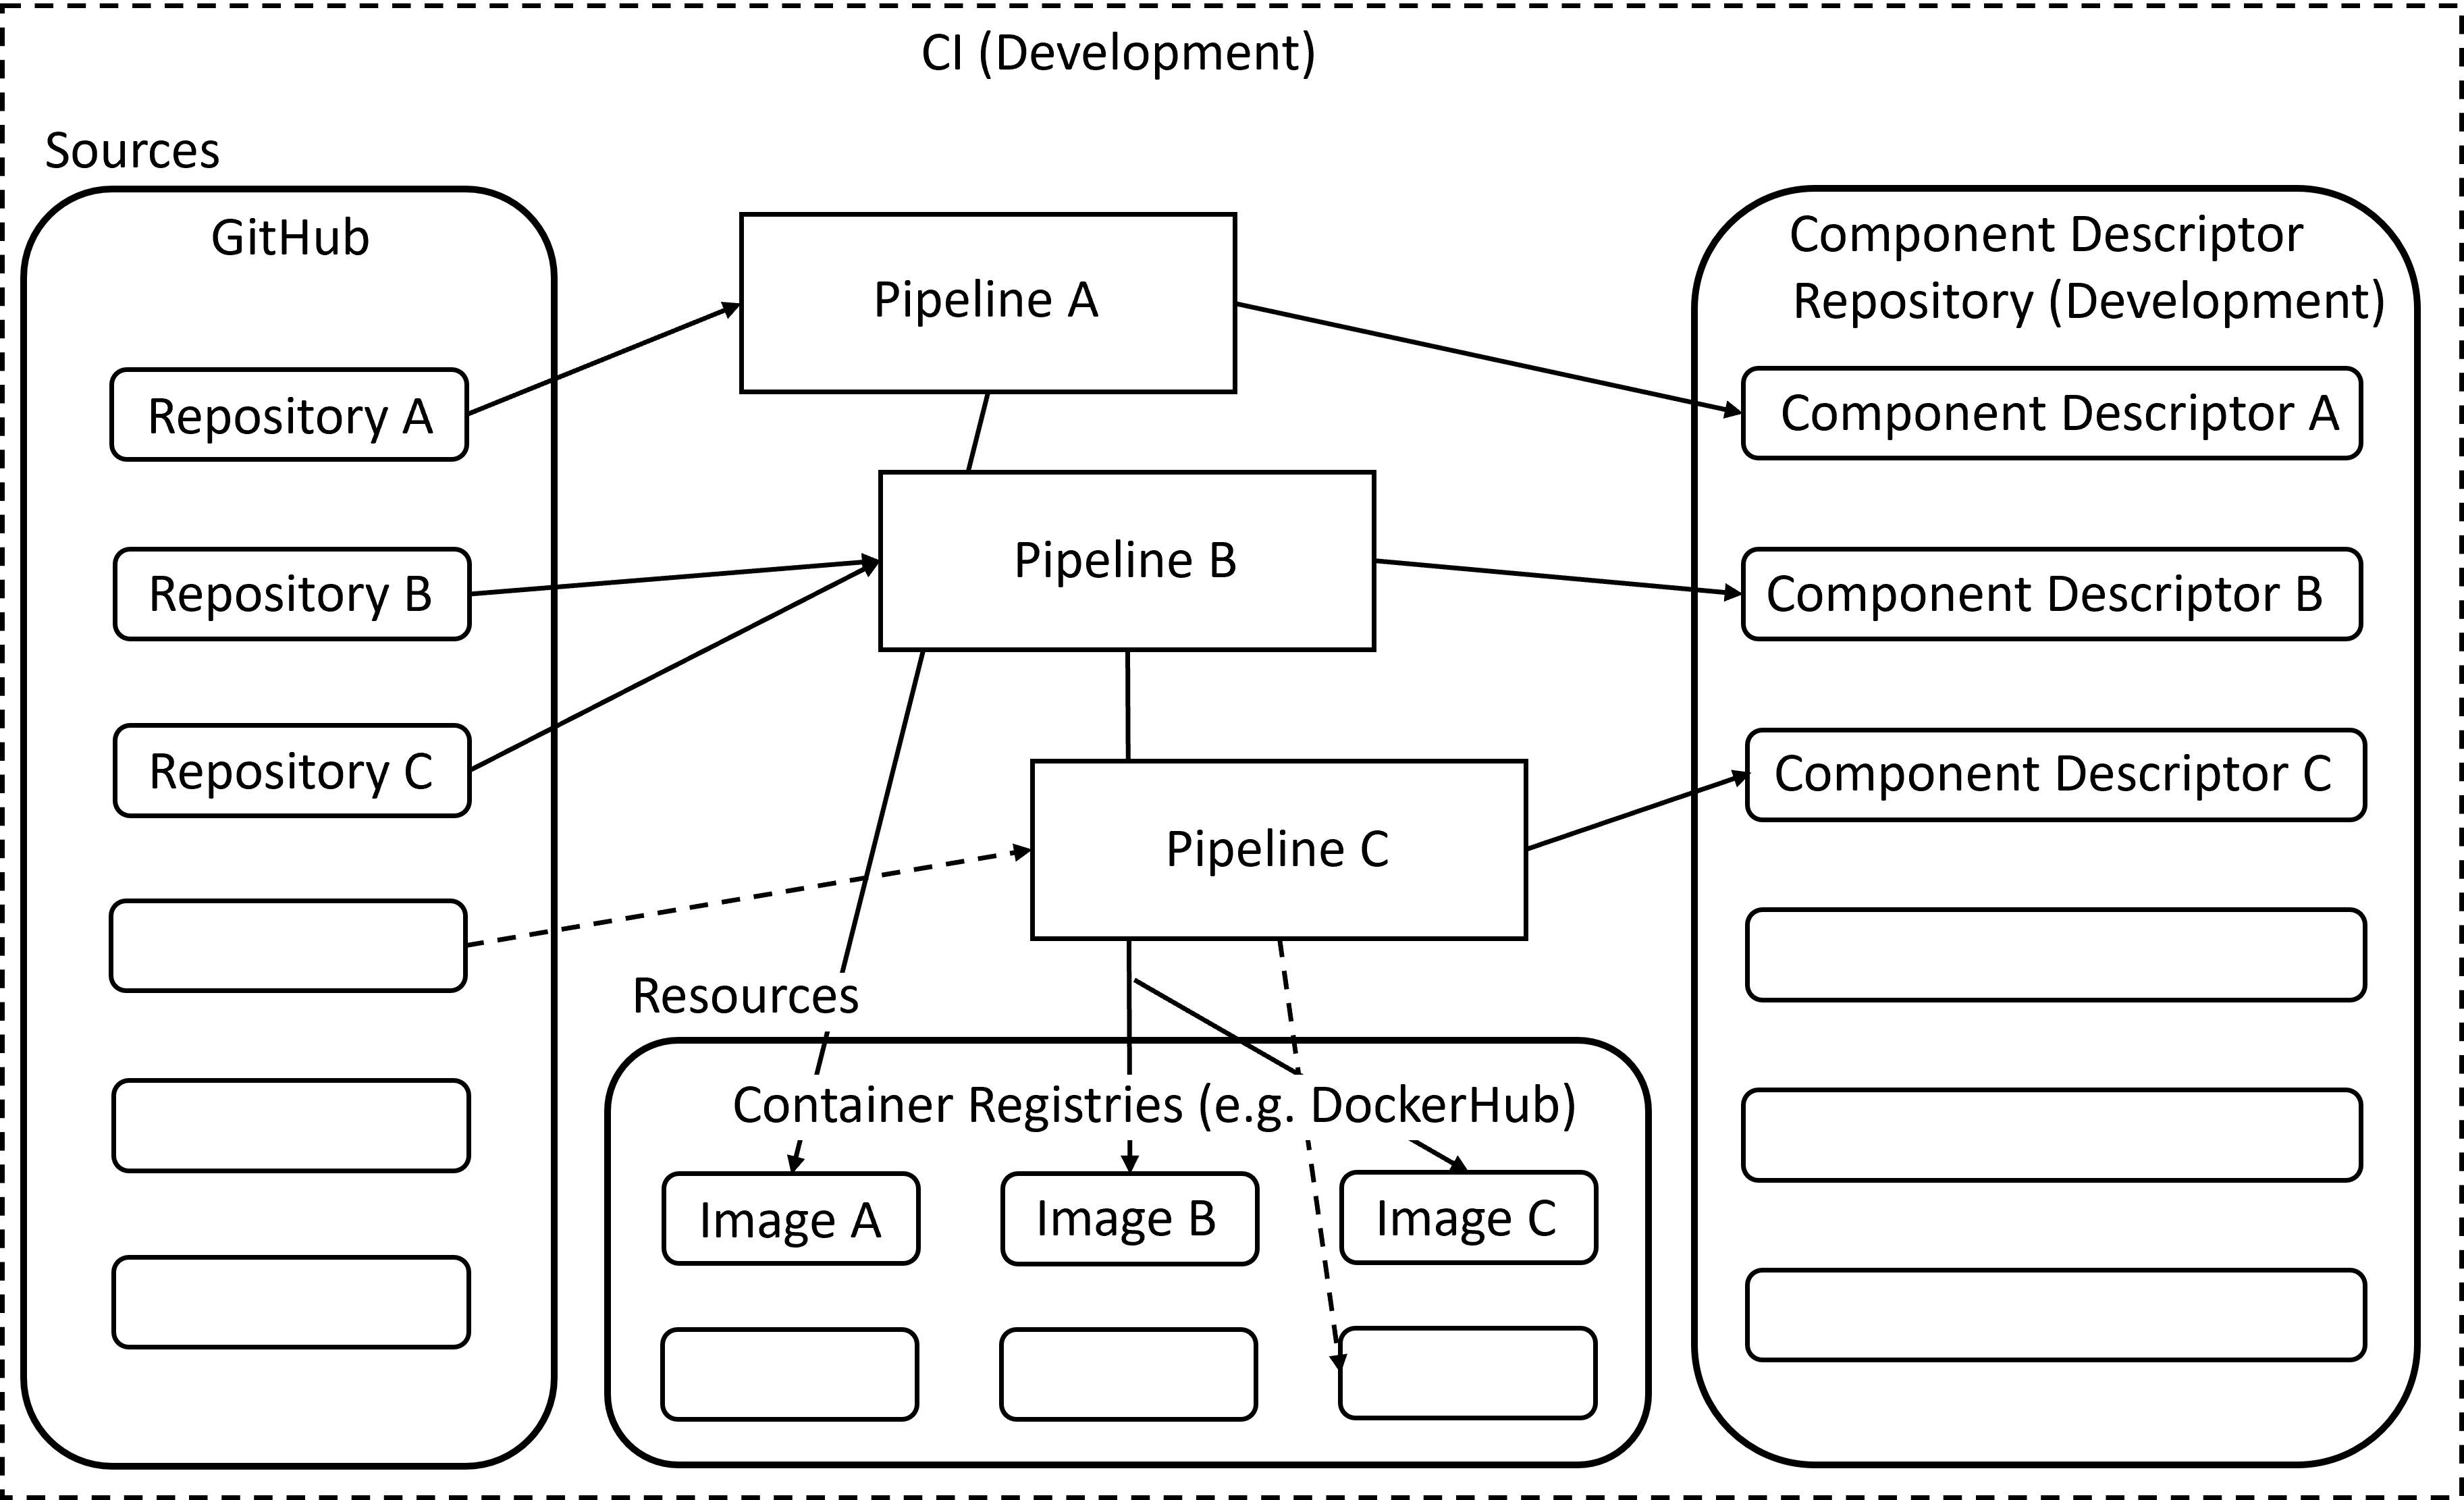
\includegraphics[scale=0.5]{gardener_ci}
	\caption[Gardener CI]{Gardener CI \source{Based on \cite{OCMInternalPresentation}}}
	\label{fig:GardenerCI}
\end{figure}

As shown, there are several sources organized in git repositories hosted on GitHub. Furthermore, there are pipelines for creating the Component Descriptors. These pipelines may build OCI Images from the sources, as indicated by the unbroken lines to Pipeline A and Pipeline B. Instead of actually building, these pipelines may also just use references to existing open source OCI Images and optionally their corresponding sources, as indicated by the dashed arrows. In fact, more than half of the OCI Images powering SAP Gardener are only referenced and not built within the pipeline. Finally, as a result of the pipeline processing, the Component Descriptors are published into the Developments Component Descriptor Repository.\\\\
The next illustration in figure \ref{fig:GardenerCD} is a representation of how this CI system is connected to the CD system.

\begin{figure}[H]
	\centering
	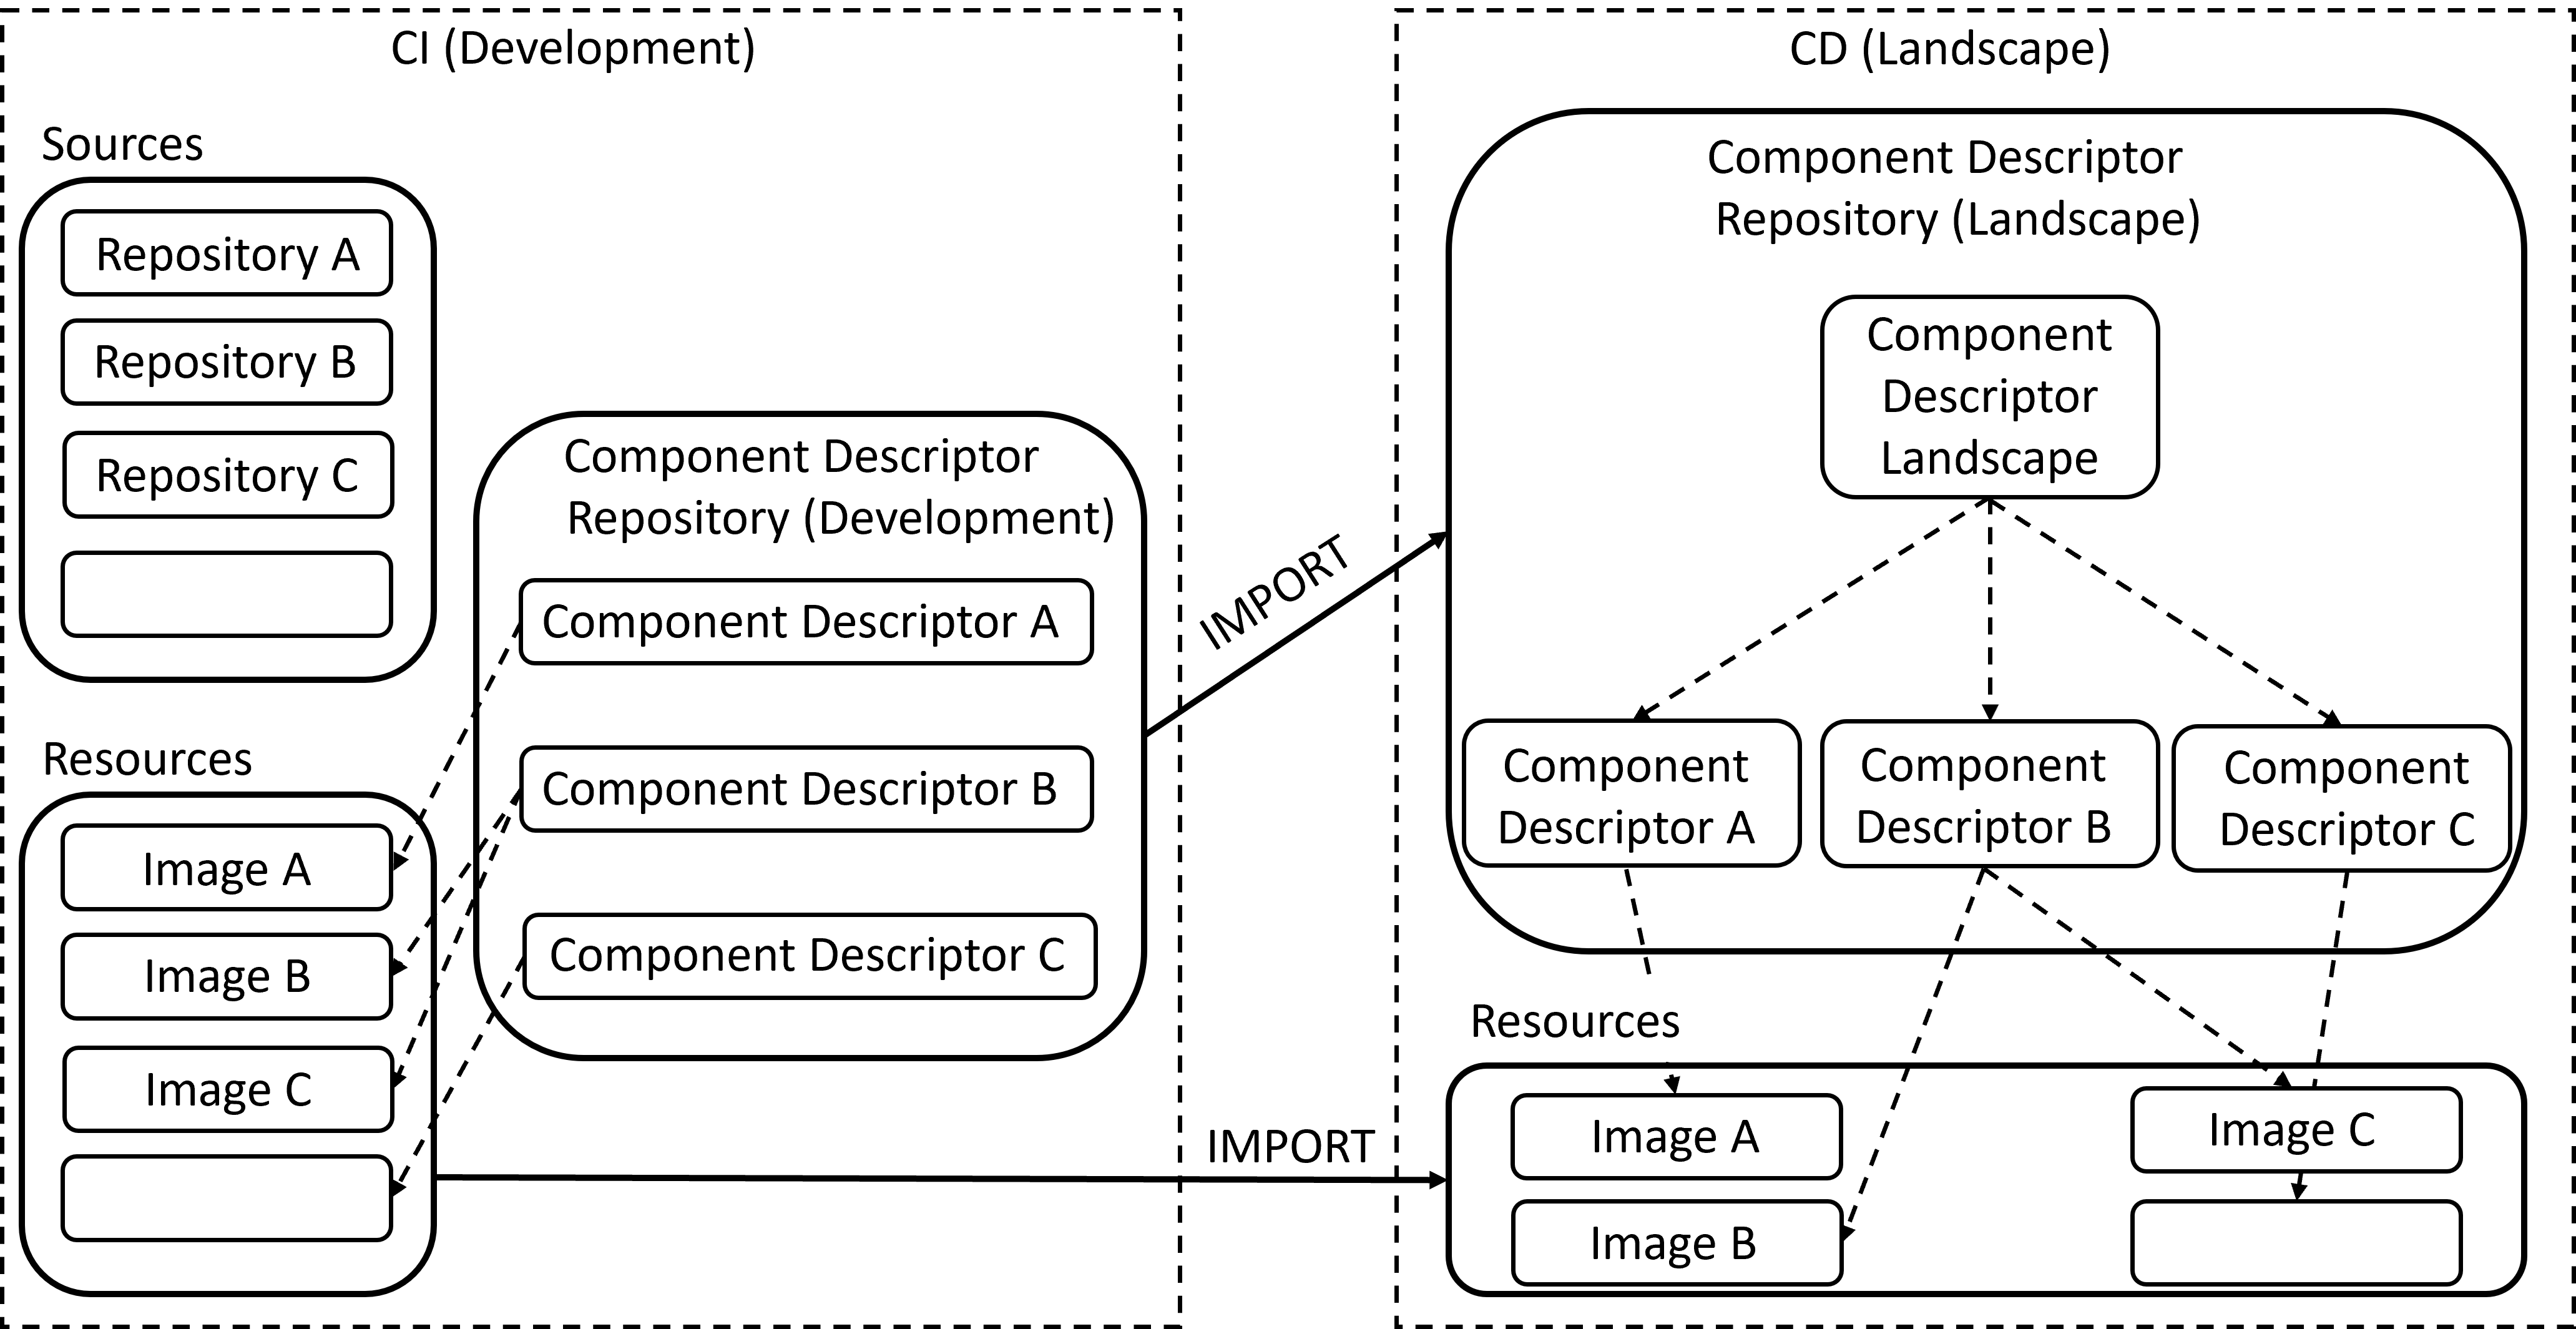
\includegraphics[scale=0.45]{gardener_cd}
	\caption[Gardener CD]{Gardener CD \source{Based on \cite{OCMInternalPresentation}}}
	\label{fig:GardenerCD}
\end{figure}
 
The left side, CI (Development) is a condensed view of figure \ref{fig:GardenerCI}. The dashed arrows represent references. Since the references to the sources stay exactly the same, these dashed arrows are omitted to avoid even more clutter.\par 
So whenever a new Component Version is released through the CI system, the CD system discovers and imports the corresponding Component Descriptors together with the referenced resources into Component Descriptor and Artifact Repositories of the respective landscape. Thereby, while essentially still referencing the same OCI Images, the access property of these Resource References of the replicated Component Descriptors is adjusted to the OCI Images in the landscapes Artifact Repository. Also, as shown in the illustration, in SAP Gardener, an additional Component Descriptor for a Landscape Component gets automatically created. It references all the Component Versions in a given snapshot of SAP Gardener. Every time a new Component Version is released in the CI system, a new Component Version of this Landscape Component is created.\par 

\begin{figure}[H]
	\centering
	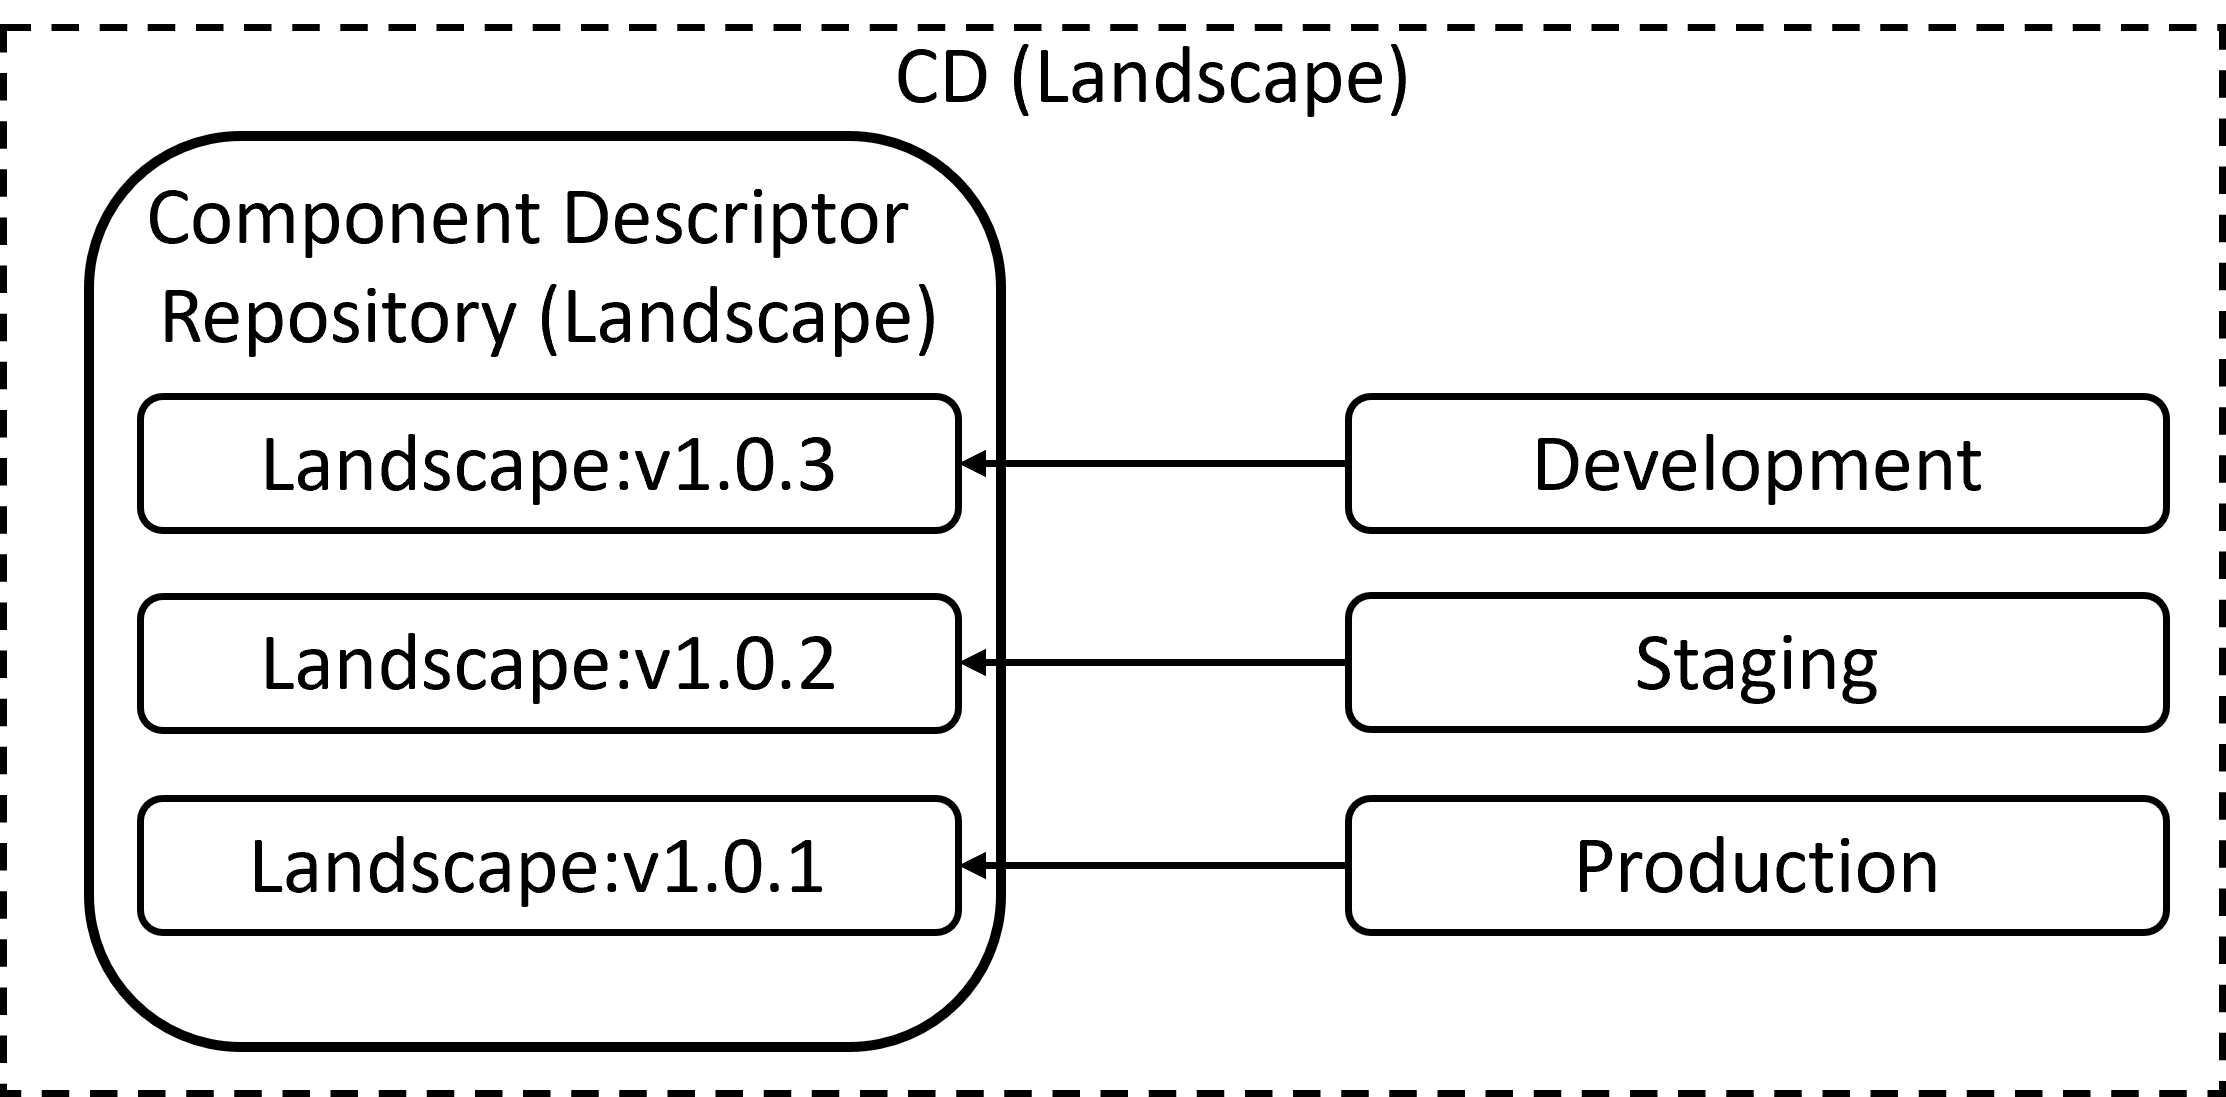
\includegraphics[scale=0.5]{gardener_deployments}
	\caption[Gardener Deployments]{Gardener Deployments \source{Based on \cite{OCMInternalPresentation}}}
	\label{fig:GardenerDeployments}
\end{figure}

Finally, figure \ref{fig:GardenerDeployments} indicates how this setup and particularly the Landscape Component is leveraged to actually deploy an instance of the SAP Gardener. Therefore, the Component References of a Landscape Component Version are traversed and the referenced resources deployed. As usual, the Production deployment is based on an older Landscape Component Version than the Development deployment. 


\section{Integration of the Security and Compliance Data Lake into the SAP Gardener Landscape}
As already indicated in the previous chapters, although the Security and Compliance Data Lake is an application for storing all kinds of metadata, the initial primary use case is storing the data resulting from compliance scans, thus dependencies, vulnerabilities and licenses. Below figure \ref{fig:DataLakeIntegration} shows the architecture designed for the integration into this complex environment of SAP Gardener.\par 
The \emph{Data Collection Service} is the central component of this architecture. Its job is to fetch all the information that shall be stored in the \emph{Data Lake}. In practice, this would be done based on policies, requiring to do such a fetching once a day or based on some kind of event. In order to actually fetch the information, the Data Collection Service sends a request to the \emph{Access Service} (1).\par
The Access Service is a transparency layer already built into the \emph{Component Repositories} as part of the OCM. Thus, if the Data Collection Service requests a set of Component Versions and their referenced Artifacts, the Access Service first fetches the corresponding Component Descriptors from the Component Repository (2). After receiving this information, the Access Service evaluates the access property in the referenced Sources and Resources and sends respective requests to the \emph{Source} and \emph{Resource Repositories} to fetch the Artifacts (3). Finally, the Access Service may return all the requested information to the Data Collection Service.\par

\begin{figure}[H]
	\centering
	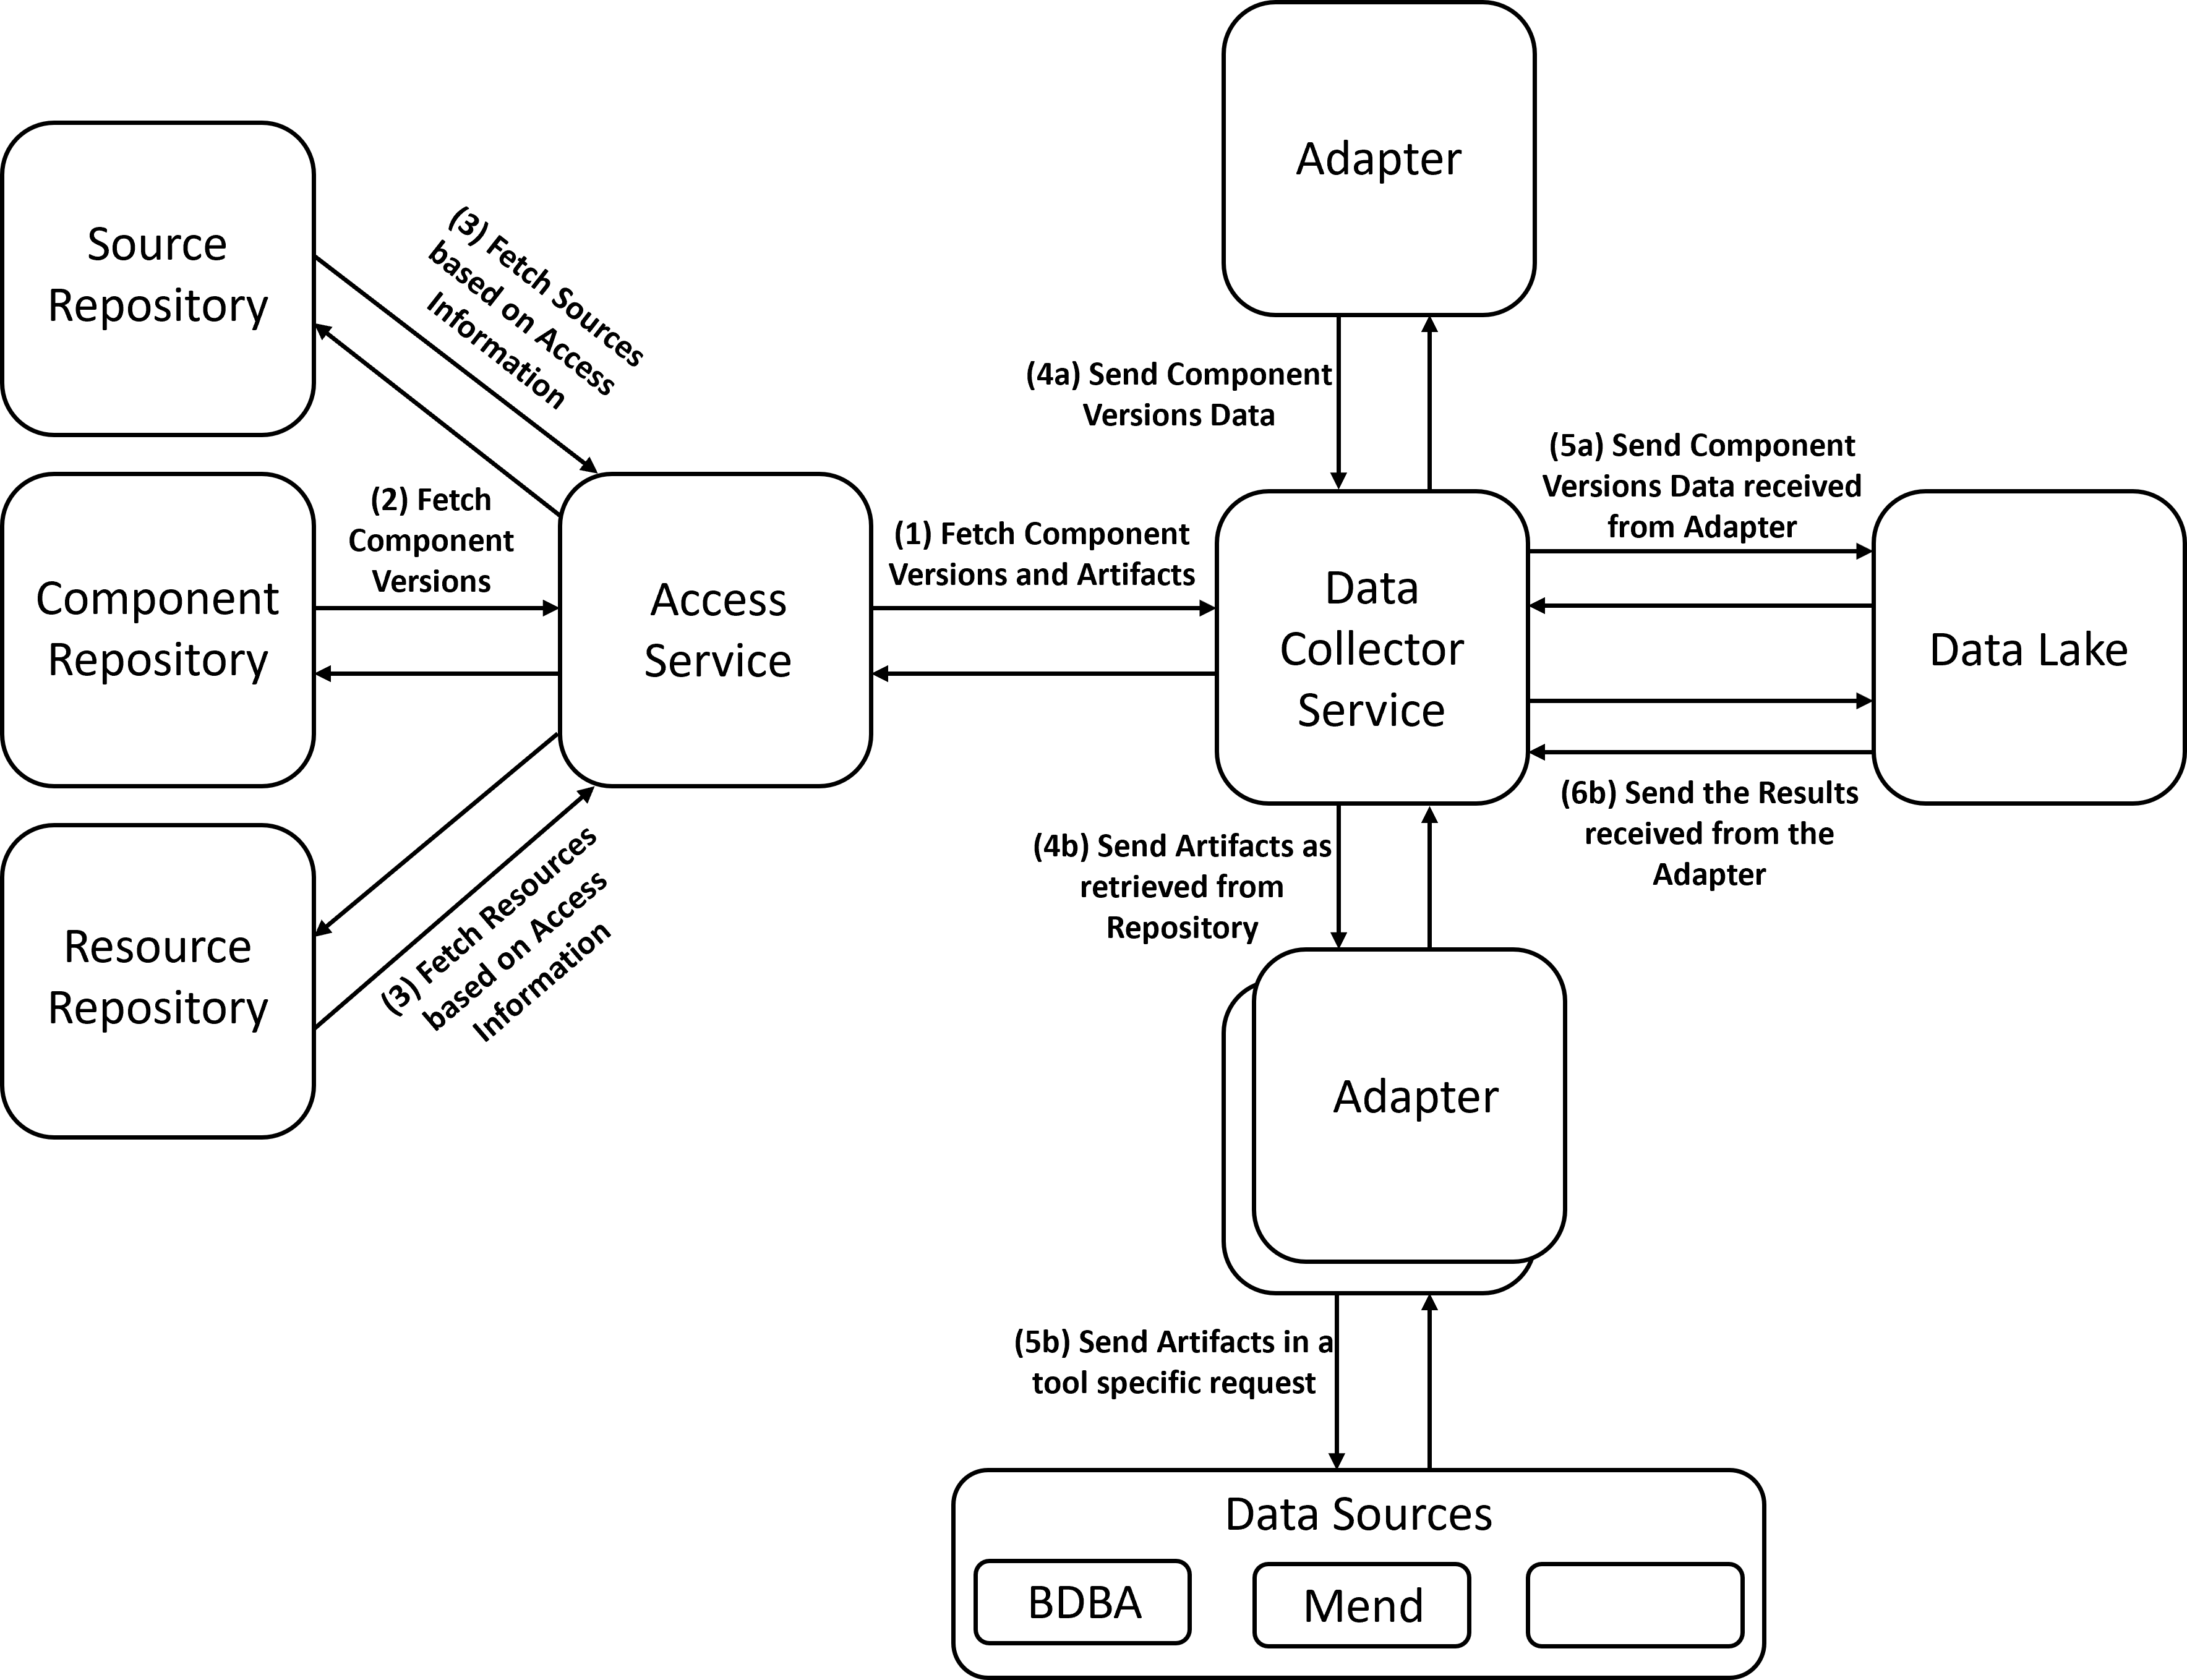
\includegraphics[scale=0.5]{datalake_integration}
	\caption[Data Lake Integration]{Data Lake Integration \source{Own representation}}
	\label{fig:DataLakeIntegration}
\end{figure}

As shown in the figure, based on this information, there are two requests flows that may be triggered by the Data Collection Service (4a) and (4b). There is no required order to this, in practice, they may even be executed in parallel. The request flow illustrated above the Data Collection Service (4a) sends the Component Versions data, so the Component Descriptors, to an \emph{Adapter} which adjusts and returns this data in the format required for the consumption by the Data Lake.\par 
The request flow below the Data Collection Service (4b) distributes the Artifacts to a set of Adapters. Here, the Adapters initially wrap the Artifacts into the format required by a specific Data Source. In this case, there would be an Adapter for each compliance scanner. Upon receipt of the scan results, these Adapters also adjust the data to the format required for consumption by the Data Lake, before returning it to the Data Collection Service.\par 
Finally, the Data Collection Service may send all the information, thus the information acquired from the Component Versions about Components, Resources, Sources and their relationships (5a) as well as the information from the scanning tools about dependencies, vulnerabilities and licenses within these Artifacts (6b) to the Data Lake.\par
There were no communication protocols mentioned so far. This is due to the facts, that it does not really matter on the conceptual level and that the final implementation of this integration architecture is out of the scope of this work. But in practice, the communication between Data Collection Service and Access Service, between Adapters and Data Sources and between Data Collection Service and Data Lake will be over HTTP. The Adapters however will most likely not be implemented as discrete services but as components within Data Collection Service and therefore communicate over shared memory. Since it is very likely that additional Data Sources shall be added later on, the important part on the conceptual level is to still logically separate the components. Thus, there should still be well defined interfaces between the Adapters and the Data Collection Service.



